\chapter{Конструкторская часть}

 При разработке алгоритмов, решающих задачи поиска расстояний Левенштейна и Дамерау-Левенштейна, можно использовать несколько различных подходов: итеративный, рекурсивный с кешированием, рекурсивный без кеширования, которые будут рассмотрены в текущем разделе.
 

\section{Алгоритм поиска расстояния Левенштейна}

На рисунке \ref{fig:leven_iter} приведена схема итеративного алгоритма поиска расстояния Левенштейна с заполнением матрицы расстояний.

\begin{figure}[h!]
	
	\centering{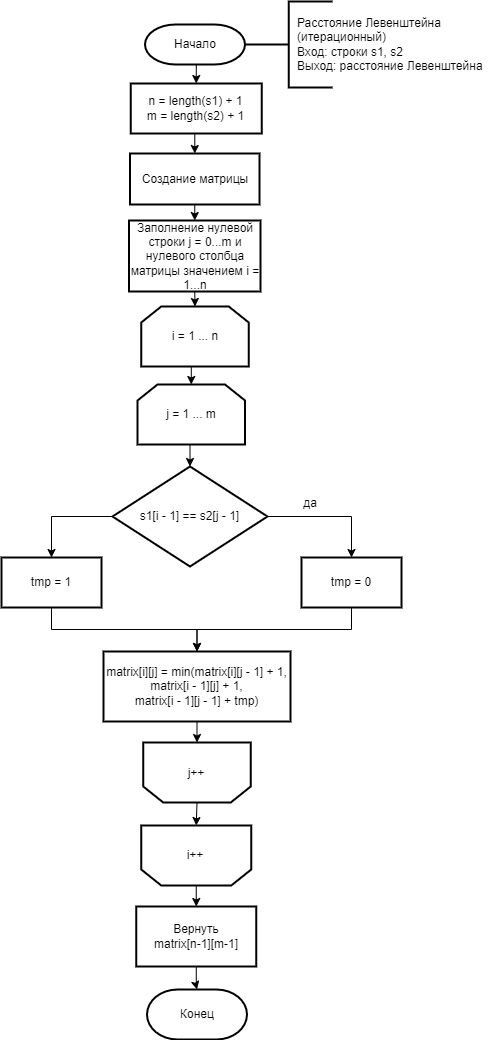
\includegraphics[scale=0.65]{inc/leven_iter.png}}
	
	\caption{Схема итеративного алгоритма поиска расстояния Левенштейна}
	
	\label{fig:leven_iter}
	
\end{figure}

%\img{220mm}{leven_iter}{Схема итеративного алгоритма поиска расстояния Левенштейна}

\section{Алгоритмы поиска расстояния Дамерау - Левенштейна}
На рисунке \ref{fig:dleven_iter} приведена схема итеративного алгоритма поиска расстояния Дамерау-Левенштейна с заполнением матрицы расстояний.

\begin{figure}[h!]
	
	\centering{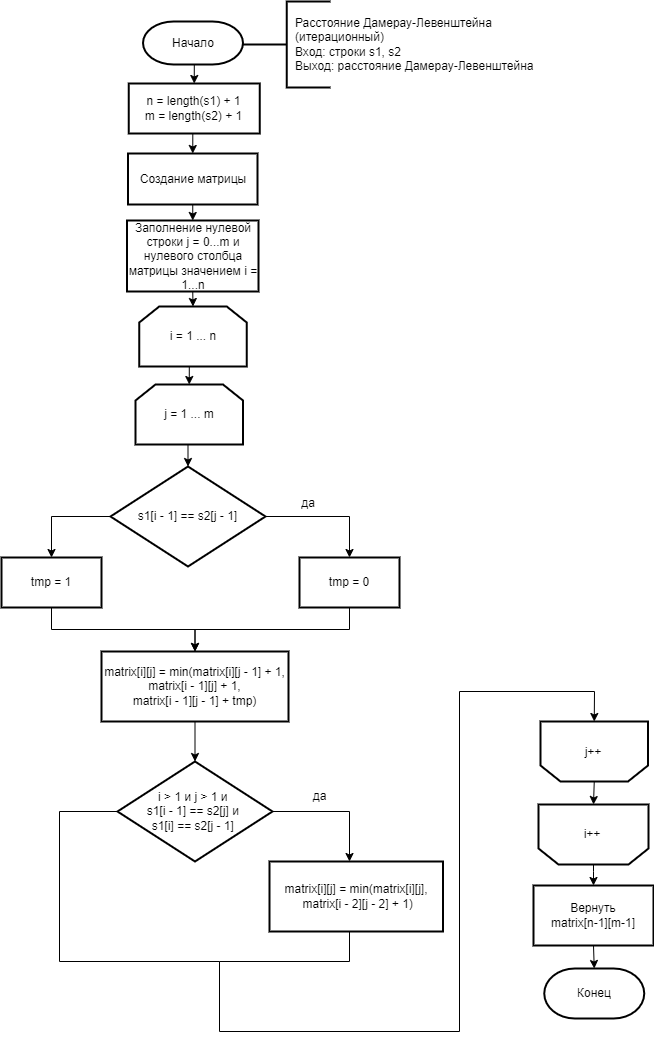
\includegraphics[scale=0.6]{inc/dleven_iter.png}}
		
	\caption{Схема итеративного алгоритма поиска расстояния Дамерау-Левенштейна}
		
	\label{fig:dleven_iter}
		
\end{figure}

%\img{180mm}{dleven_iter}{Схема итеративного алгоритма поиска расстояния Дамерау-Левенштейна}

На рисунке \ref{fig:dleven_rec1} приведена схема рекурсивного алгоритма поиска расстояния Дамерау-Левенштейна без кеширования.

\begin{figure}[h!]
	
	\centering{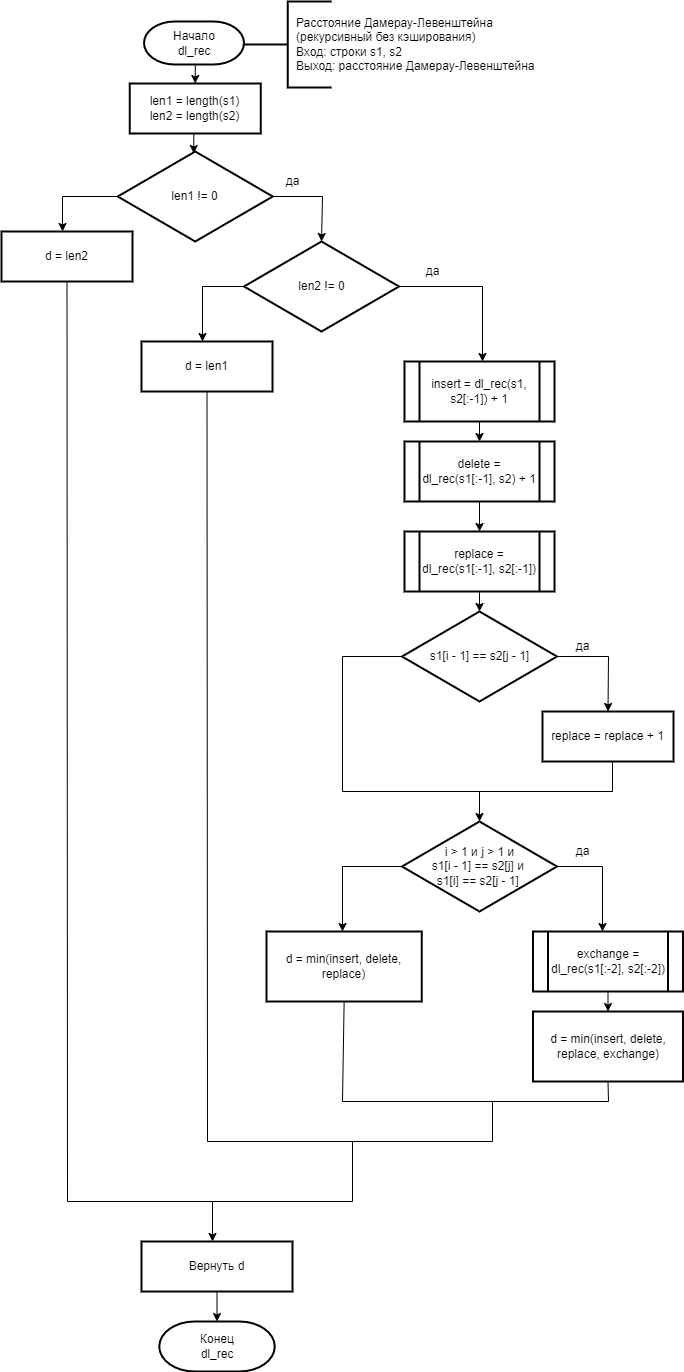
\includegraphics[scale=0.5]{inc/dleven_rec1.png}}
		
	\caption{Схема рекурсивного алгоритма поиска расстояния Дамерау-Левенштейна без кеширования}
		
	\label{fig:dleven_rec1}
		
\end{figure}

%\img{220mm}{l_recursion_matrix}{Схема рекурсивного алгоритма поиска расстояния Дамерау-Левенштейна без кеширования}

На рисунках \ref{fig:dleven_rec_cash1} $-$ \ref{fig:dleven_rec_cash3} приведена схема рекурсивного алгоритма поиска расстояния Дамерау-Левенштейна с кешированием.

\begin{figure}[h!]
	
	\centering{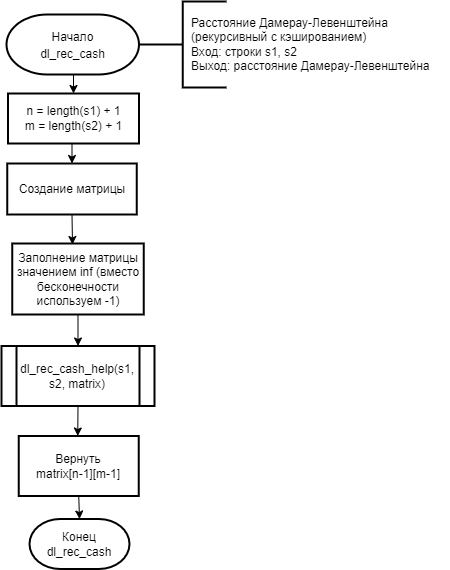
\includegraphics[scale=0.9]{inc/dleven_rec_cash1.png}}
		
		\caption{Схема рекурсивного алгоритма поиска расстояния Дамерау-Левенштейна с кешированием}
		
		\label{fig:dleven_rec_cash1}
		
	\end{figure}

%\img{220mm}{Dl_recursion}{Схема рекурсивного алгоритма поиска расстояния Дамерау-Левенштейна с кешированием}

\begin{figure}[h!]
	
	\centering{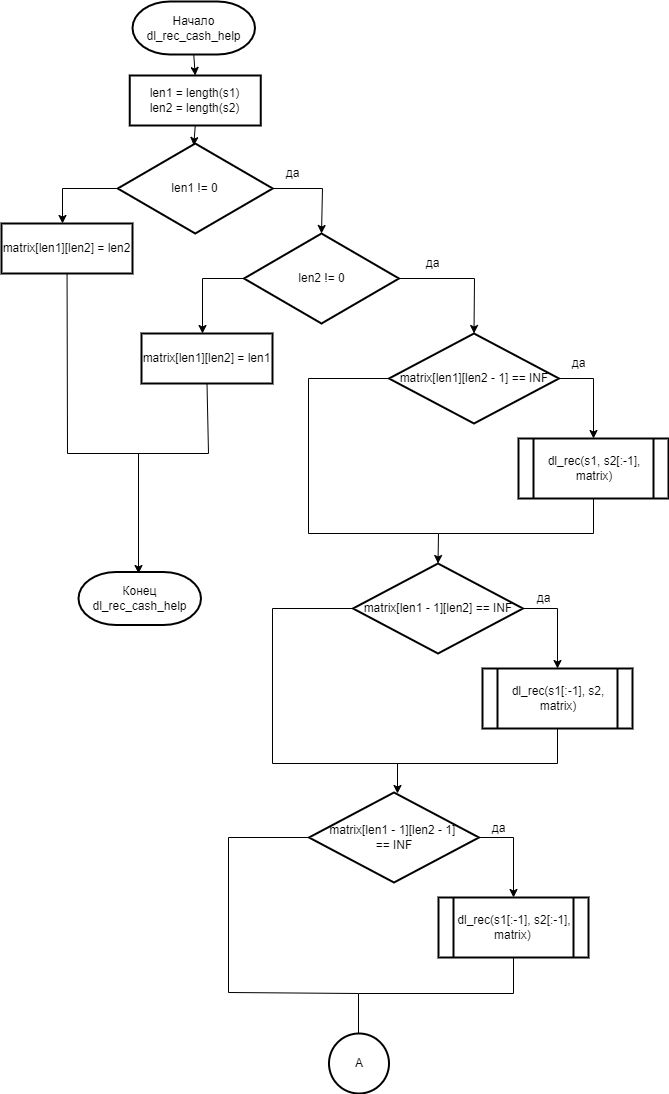
\includegraphics[scale=0.6]{inc/dleven_rec_cash2.png}}
		
		\caption{Схема рекурсивного алгоритма поиска расстояния Дамерау-Левенштейна с кешированием}
		
		\label{fig:dleven_rec_cash2}
		
	\end{figure}

\begin{figure}[h!]
	
	\centering{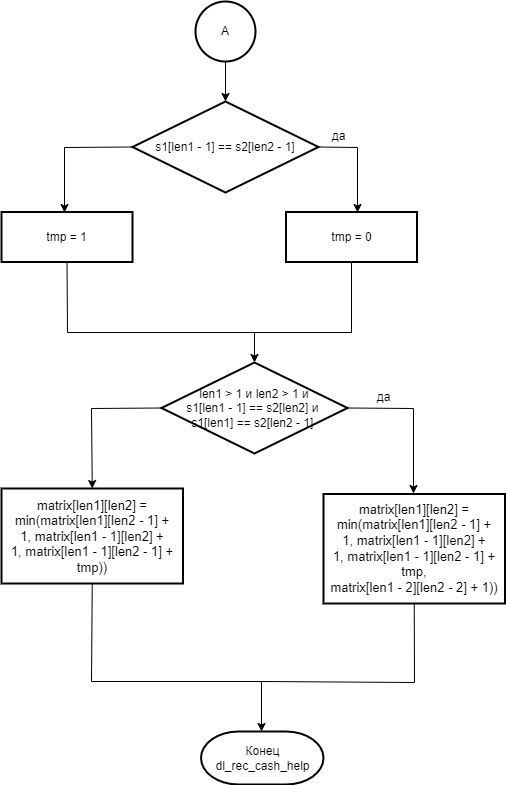
\includegraphics[scale=0.7]{inc/dleven_rec_cash3.png}}
		
		\caption{Схема рекурсивного алгоритма поиска расстояния Дамерау-Левенштейна с кешированием}
		
		\label{fig:dleven_rec_cash3}
		
	\end{figure}

\section*{Вывод}

В данном разделе Были разработаны схемы алгоритмов, которые позволяютс помощью различных подходов находить расстояния Левенштейна и Дамерау-Левенштейна.

